\section{Auswertung}
\label{sec:Auswertung}

Die Maße, also Durchmesser $d$ bzw. Kantenlänge $a$ des eckigen Stabes mit quadratischem Querschnitt, Masse $m$ und Länge $l$ der Stäbe betragen

\begin{equation}
  a_{eckig} = 10,1 \pm 0,05mm \\
  m_{eckig} = 167,9 \pm 0,1g \\
  l_{eckig} = 620 \pm 0,05mm\\
\end{equation}

\begin{equation}
  d_{rund} = 10,1 \pm 0,05mm \\
  m_{rund} = 390,6 \pm 0,1g \\
  l_{rund} = 592 \pm 0,05mm \\
\end{equation}

Der eckige Stab besteht aus Aluminium, der runde aus Messing.\\
Um die Elastizitätsmodule zu bestimmen, müssen zuerst die Flächenträgheitsmomente $I$ nach --- errechnet werden.\\
Für den quadratischen Querschnitt mit Kantenlänge a ergibt sich die Formel $I_Q = \frac{a^4}{12}$ und 
für den kreisförmigen Querschnitt
$I_K = \frac{\pi r^4}{4}$. \\
Somit kommt man, die Gaußsche Fehlerfortpflanzung hinzugezogen, zu folgenden Flächenträgheitsmomenten:

\begin{equation}
  I_{rund} = \frac{\pi (0.5\cdot 10^{-3}m)^4}{4} = 4,91 \cdot 10^{-14}m^4 \quad 
  \textrm{und} \quad I_{eckig} = \frac{(1 \cdot 10^{-3}m)^4}{12} = 8,34 \cdot 10^{-14}m^4
\end{equation}

mit 

\begin{equation}
  \varDelta I_{rund} =  \sqrt{ (\frac{\partial I_{rund}}{\partial r})^2 \cdot (\varDelta r)^2} =  \\
  \textrm{und} \quad \varDelta I_{eckig} = \sqrt{ (\frac{\partial I_{eckig}}{\partial a})^2 } = 
\end{equation}



\subsection{Einseitige Einspannung}
\label{sec:Einseitige Einspannung}



\subsubsection{Runder Stab}
\label{sec:Runder Stab}

\begin{table}[H]
  \centering
  \caption{Es wurden die Zeiten wieder verdoppelt, um sich, wie die Apparaturkonstanten, auf die Strecke 
  von $\symup{\Delta}s=100\unit{\milli\meter}$ zu beziehen.}
  \begin{tabular}{ccccc}
    \toprule
    {$T \mathbin{/} \unit{\kelvin}$} &
    {$\bar{t}_{hin} \mathbin{/} \unit{\second}$} &
    {$\bar{t}_{zur} \mathbin{/} \unit{\second}$} &
    {$\eta_{hin} \mathbin{/} \unit{\milli\pascal\second}$} &
    {$\eta_{zur} \mathbin{/} \unit{\milli\pascal\second}$} \\
    \midrule
    298.15 & 70.34          & 70.72          & 1.1386$\pm$0.0473 & 1.1705$\pm$0.0412 \\
    302.15 & 65.15$\pm$0.25 & 67.06          & 1.0554$\pm$0.0440 & 1.1107$\pm$0.0391 \\
    305.15 & 59.61$\pm$0.31 & 59.89$\pm$0.37 & 0.9657$\pm$0.0404 & 0.9922$\pm$0.0354 \\
    307.15 & 58.73$\pm$0.49 & 58.84$\pm$0.26 & 0.9528$\pm$0.0404 & 0.9740$\pm$0.0346 \\
    309.15 & 57.16$\pm$0.42 & 57.85$\pm$0.39 & 0.9273$\pm$0.0391 & 0.9595$\pm$0.0344 \\
    311.15 & 54.31$\pm$0.59 & 55.39$\pm$0.39 & 0.8821$\pm$0.0379 & 0.9199$\pm$0.0330 \\
    313.15 & 51.7$\pm$0.26  & 52.82$\pm$0.46 & 0.8398$\pm$0.0351 & 0.8772$\pm$0.0318 \\
    315.15 & 50.82$\pm$0.02 & 50.82$\pm$0.62 & 0.8255$\pm$0.0343 & 0.8440$\pm$0.0314 \\
    317.15 & 48.61$\pm$0.53 & 48.54$\pm$0.14 & 0.7907$\pm$0.0340 & 0.8073$\pm$0.0285 \\
    319.15 & 47.34$\pm$0.26 & 47.64$\pm$0.34 & 0.7701$\pm$0.0323 & 0.7923$\pm$0.0284 \\
    321.15 & 45.59$\pm$0.43 & 45.66$\pm$0.14 & 0.7427$\pm$0.0316 & 0.7606$\pm$0.0269 \\
    323.15 & 44.2$\pm$1.24  & 44.4$\pm$0.22  & 0.7201$\pm$0.0361 & 0.7396$\pm$0.0263 \\
    \bottomrule
  \end{tabular}
  \label{tab:Tabelle1}
\end{table}

\begin{figure}
  \centering
  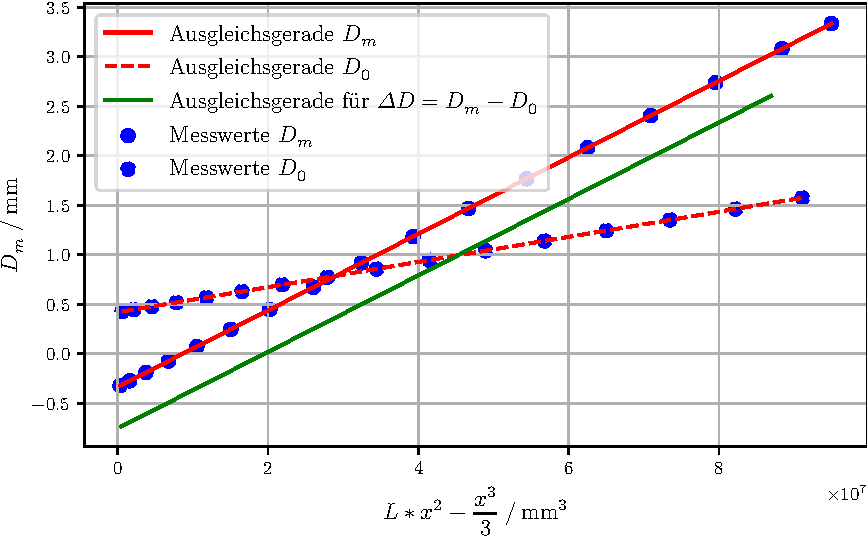
\includegraphics{plot_messing_einseitig.pdf}
  \caption{Plot.}
  \label{fig:plot}
\end{figure}

\subsubsection{Eckiger Stab}
\label{sec:Eckiger Stab}


\begin{figure}
  \centering
  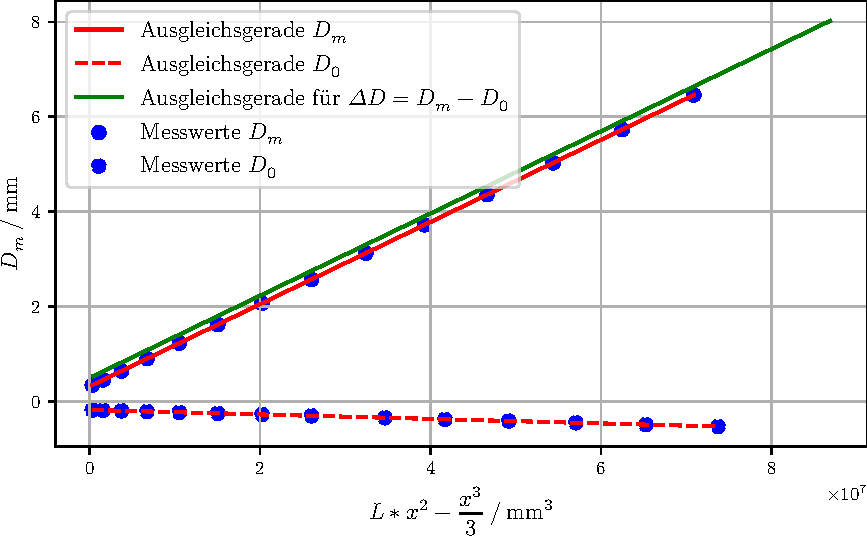
\includegraphics{plot_alu_einseitig.pdf}
  \caption{Plot.}
  \label{fig:plot_alu_einseitig}
\end{figure}




\subsection{Beidseitige Auflage}
\label{sec:Beidseitige Auflage}



\begin{table}[H]
  \centering
  \caption{Die Werte für die beidseitige Auflage bei Messung am runden Messingstab von rechts bis zur Mitte}
  \begin{tabular}{ccccc}
    \toprule
    {$x \mathbin{/} \unit{\milli\metre}$} &
    {$D_0(x) \mathbin{/} \unit{\milli\metre}$} &
    {$D_m(x) \mathbin{/} \unit{\milli\metre}$} \\
    \midrule
    30 & 0.01 & 0.20  \\  
    60 & 0.04 & 0.48 \\
    90 & 0.09 & 0.71 \\
    120 & 0.13 & 0.93 \\
    150 & 0.19 & 1.14 \\
    180 & 0.22 & 1.32 \\
    210 & 0.26  & 1.46 \\
    240 & 0.33 & 1.58 \\
    
    \bottomrule
  \end{tabular}
  \label{tab:Tabelle3}
\end{table}



\begin{table}[H]
  \centering
  \caption{Die Werte für die beidseitige Auflage bei Messung am runden Messingstab von rechts bis zur Mitte}
  \begin{tabular}{ccccc}
    \toprule
    {$x \mathbin{/} \unit{\milli\metre}$} &
    {$D_0(x) \mathbin{/} \unit{\milli\metre}$} &
    {$D_m(x) \mathbin{/} \unit{\milli\metre}$} \\
    \midrule
    0 & 0.00 & 0.10
    30 & 0.09 & 0.20  \\  
    60 & 0.15 & 0.32 \\
    90 & 0.24 & 0.41 \\
    120 & 0.32 & 0.50 \\
    150 & 0.35 & 0.58 \\
    180 & 0.42 & 0.65 \\
    210 & 0.45 & 0.70 \\
    240 & 0.52 & 0.71 \\
    \bottomrule
  \end{tabular}
  \label{tab:Tabelle3}
\end{table}








\begin{figure}
  \centering
  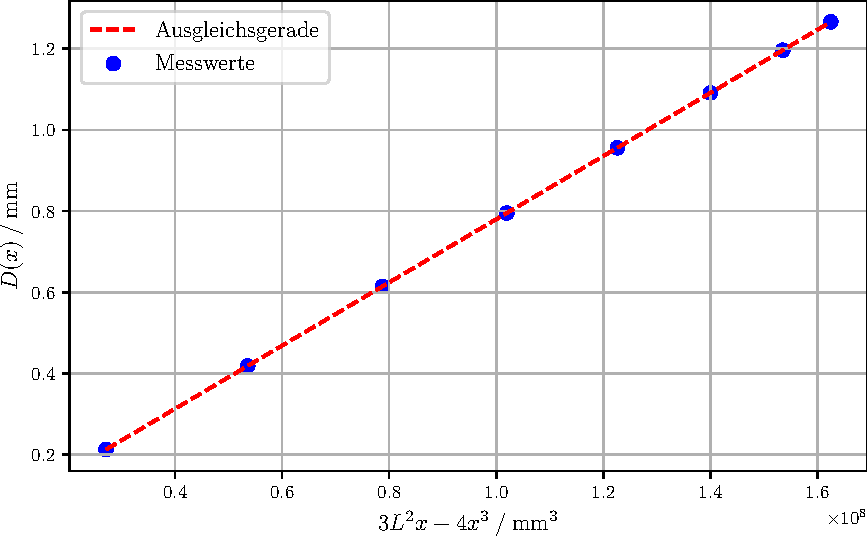
\includegraphics{plot_beidseitig_rechts.pdf}
  \caption{Die lineare Regression für die Messung am beidseitig aufliegenden, runden Messingstab von rechts}
  \label{fig:plot_beidseitig_rechts}
\end{figure}

\begin{figure}
  \centering
  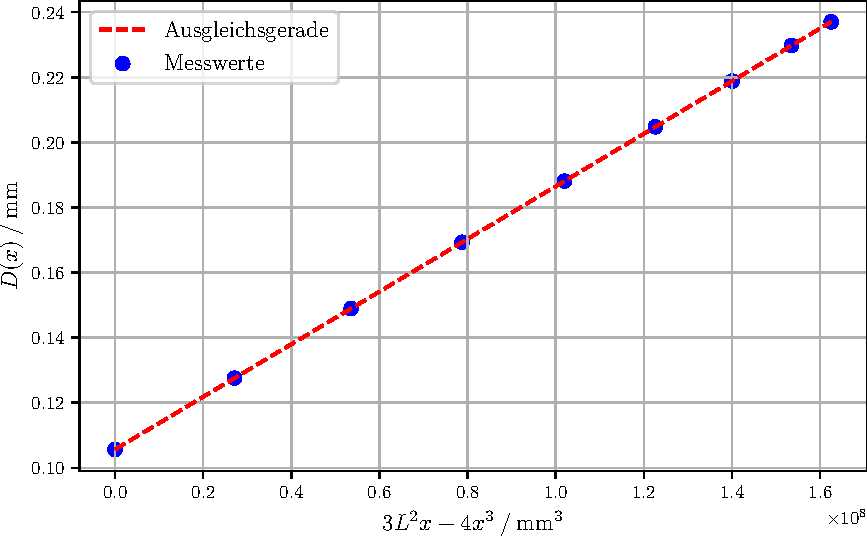
\includegraphics{plot_beidseitig_links.pdf}
  \caption{Die lineare Regression für die Messung am beidseitig aufliegenden, runden Messingstab von links}
  \label{fig:plot_beidseitig_links}
\end{figure}


Siehe \autoref{fig:plot}! 
